%\title{LaTeX Portrait Poster Template}
%%%%%%%%%%%%%%%%%%%%%%%%%%%%%%%%%%%%%%%%%
% a0poster Portrait Poster
% LaTeX Template
% Version 1.0 (22/06/13)
%
% The a0poster class was created by:
% Gerlinde Kettl and Matthias Weiser (tex@kettl.de)
% 
% Adapter by Jens Buysse for Hogeschool Gent
% This template has been downloaded from:
% http://www.LaTeXTemplates.com
%
% License:
% CC BY-NC-SA 3.0 (http://creativecommons.org/licenses/by-nc-sa/3.0/)
%
%%%%%%%%%%%%%%%%%%%%%%%%%%%%%%%%%%%%%%%%%

%----------------------------------------------------------------------------------------
%	PACKAGES AND OTHER DOCUMENT CONFIGURATIONS
%----------------------------------------------------------------------------------------

\documentclass[a0,portrait]{a0poster}

\usepackage{multicol} % This is so we can have multiple columns of text side-by-side
\columnsep=100pt % This is the amount of white space between the columns in the poster
\columnseprule=3pt % This is the thickness of the black line between the columns in the poster

\usepackage[svgnames]{xcolor} % Specify colors by their 'svgnames', for a full list of all colors available see here: http://www.latextemplates.com/svgnames-colors

\usepackage{times} % Use the times font
%\usepackage{palatino} % Uncomment to use the Palatino font

\usepackage{graphicx} % Required for including images
\graphicspath{{figures/}} % Location of the graphics files
\usepackage{booktabs} % Top and bottom rules for table
\usepackage[font=small,labelfont=bf]{caption} % Required for specifying captions to tables and figures
\usepackage{amsfonts, amsmath, amsthm, amssymb} % For math fonts, symbols and environments
\usepackage{wrapfig} % Allows wrapping text around tables and figures
\usepackage[export]{adjustbox}

\begin{document}

%----------------------------------------------------------------------------------------
%	POSTER HEADER 
%----------------------------------------------------------------------------------------

% The header is divided into two boxes:
% The first is 75% wide and houses the title, subtitle, names, university/organization and contact information
% The second is 25% wide and houses a logo for your university/organization or a photo of you
% The widths of these boxes can be easily edited to accommodate your content as you see fit

\begin{minipage}[t]{0.75\linewidth}
\VeryHuge \color{HoGentAccent1} \textbf{Monitoring voor Kubernetes en Docker} \color{Black}\\ % Title
\Huge\textit{}\\[2.4cm] % Subtitle
\huge \textbf{Troch Olivier, Bert Van Vreckem}\\[0.5cm] % Author(s)
\huge Hogeschool Gent, Valentin Vaerwyckweg 1, 9000 Gent\\[0.4cm] % University/organization
\Large \texttt{olivier.troch.w2257@student.hogent.be} \\
\end{minipage}
%
\begin{minipage}[t]{0.25\linewidth}

\includegraphics[width=13cm,right]{figures/HOGENT_Logo_Pos_rgb.png} 

\end{minipage}

\vspace{1cm} % A bit of extra whitespace between the header and poster content

%----------------------------------------------------------------------------------------

\begin{multicols}{2} % This is how many columns your poster will be broken into, a portrait poster is generally split into 2 columns

%----------------------------------------------------------------------------------------
%	ABSTRACT
%----------------------------------------------------------------------------------------
\color{HoGentAccent1} % Navy color for the abstract
%
\begin{abstract}
Kosten besparen en winst verhogen zijn legitieme zakelijke doelstellingen. Preventie door monitoring betekent dat er minder geld wordt uitgegeven in vergelijking met de kosten van oplossingen voor problemen die zich plotseling kunnen voordoen. Helaas wordt monitoring van een infrastructuur vaak onderschat en steeds eerder als een kost gezien dan als een opbrengst. IT-afdelingen besteden vaker tijd aan het reageren op de onverwachte problemen of fouten dan aan het voorkomen ervan. Hierdoor lijkt het van goed belang dat de basisconcepten van monitoring in het lessenpakket verwerkt worden, zodat het nut van monitoring wordt meegegeven en zich gemakkelijker in de bedrijfswereld kan mengen.
\end{abstract}
%----------------------------------------------------------------------------------------
%	INTRODUCTION
%----------------------------------------------------------------------------------------

\color{HoGentAccent1} 
\section*{Introductie}
\color{black}
\color{black}

HOGENT kan helaas niet beschikken over alle mogelijke technologieën die bestaan in de informatica wereld. Toch zijn er bepaalde onderwerpen die onderdeel van het lessenpakket zouden moeten zijn. Monitoring van de infrastructuur is hier één van en meer specifiek de monitoring van een containerorkestratie. Containerisatie vindt in een recordtempo zijn weg naar de data-omgeving van de ondernemingen. Het gemak waarmee containerplatformen zoals Docker kunnen worden ingezet, suggereert dat ze de dominantste architectuur zijn en zullen blijven. De uitdaging is om goede monitoring voor deze containers op te stellen. Containers zijn zeer vluchtig in ontstaan en net zo snel in het verdwijnen. Zoals te verwachten, zullen traditionele monitoringsplatforms die vooral gebaseerd zijn op virtualisatie, niet voldoende zijn.  Om het monitoringproces te vergemakkelijken kan er beroep gedaan worden op monitoringtools die gecreëerd of aangepast zijn om een containerorkestratie te kunnen monitoren.
%----------------------------------------------------------------------------------------
%	GEOLOGY
%----------------------------------------------------------------------------------------

\color{Black} % DarkSlateGray color for the rest of the content
\color{HoGentAccent1} 
\section*{Onderzoek}
\color{black}

Via de state-of-the-art werd gezocht naar een aantal tools die geschikt zijn voor het monitoren van een containerorkestratie waarna aan de hand van een requirements-analyse die gevonden tools vergeleken werden met elkaar. Nadien werd een Proof-of-Concept opgesteld waarin de werking van de, in dit onderzoek, beste tool toegepast werd. Door het onderzoek werd beslist dat een combinatie van Prometheus en Grafana geschikt was. In deze proof-of-concept werd gebruik gemaakt van standaard dashboards, maar ook van het importeren en creëren van eigen dashboards om de metrieken van de containers te weergeven en analyseren.

%\color{HoGentAccent1} 
%\section*{Sectie met figuur}
%\color{black}


%\begin{center}\vspace{1cm}
%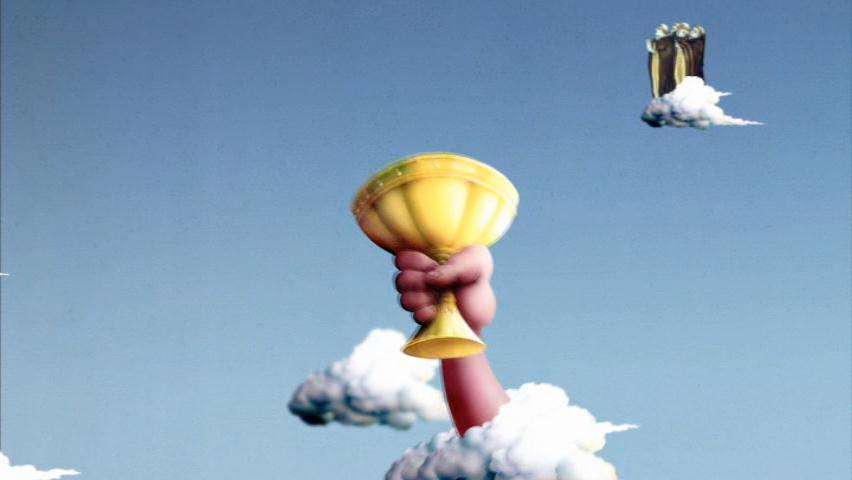
\includegraphics[width=1.0\linewidth]{grail}
%\captionof{figure}{\color{HoGentAccent5} He hasn't got shit all over him. The nose? %Where'd you get the coconuts? What do you mean? We shall say 'Ni' again to you, if you %do not appease us}
%\end{center}\vspace{1cm}

%------------------------------------------------



\color{HoGentAccent1} 
\section*{Conclusies}
\color{black}

Door het uitvoeren van de requirements-analyse zijn 3 tools overgebleven die als geschikt verklaard waren. Op basis van de analyse waren deze 3 tools praktisch hetzelfde en om de finale beslissing te maken werd de monitoringcommunity geraadpleegd. Hieruit bleek dat Prometheus de tool was die met voorsprong uitblonk. Achteraf werden, aan de hand van een stappenplan, alle opties uitgelegd die nodig waren om een antwoord op de onderzoeksvraag en deelvragen te formuleren. Door het gebruik van de Helm-tool was de installatie van de tool relatief eenvoudig waardoor de toekomstige studenten de opstelling makkelijk zullen kunnen nabootsen om snel aan de slag te kunnen. 

%----------------------------------------------------------------------------------------
%	FORTHCOMING RESEARCH
%----------------------------------------------------------------------------------------
\color{HoGentAccent1} 
\section*{Toekomstig onderzoek}
\color{black}

Bijkomend onderzoek kan nodig zijn om de hoofdonderzoeksvraag of deelvragen uit te breiden, om meer functies aan bod te brengen dan degene die werden meegegeven in het huidige onderzoek. Indien het de bedoeling is om dit onderzoek te gebruiken als basis voor het introduceren van andere, nieuwe technologieën kan dit betekenen dat dit onderzoek het einde nog niet bereikt heeft.


%----------------------------------------------------------------------------------------

\end{multicols}
\end{document}